\documentclass[11pt,twocolumn]{article}

% --- Codificación y lenguaje ---
\usepackage[T1]{fontenc}
\usepackage[utf8]{inputenc}
\usepackage[spanish]{babel}

% --- Matemática y fuentes ---
\usepackage{amsfonts, amssymb, amsthm}
\usepackage{derivative}
\usepackage{physics} 

% --- Gráficos y tablas ---
\usepackage{graphicx}
\usepackage{caption}        % <-- primero caption
\usepackage{subcaption}     % <-- luego subcaption
\usepackage{booktabs}

% --- Varios útiles ---
\usepackage[margin=2cm]{geometry}
\usepackage{enumitem}
\usepackage{csquotes}
\usepackage{cuted}          % para elementos a dos columnas (opcional)
\usepackage{stackrel}
%\usepackage{microtype}      % cargar una sola vez
\usepackage{float}
\usepackage{placeins}
% \usepackage{nameref}      % NO necesario: hyperref ya define \nameref
\usepackage[dvipsnames]{xcolor}
\usepackage{tikz}
\usetikzlibrary{calc}

% --- Bibliografía (BibTeX + apacite) ---
\usepackage[backend=biber,style=apa,language=spanish]{biblatex}
\addbibresource{referencias.bib} % tu archivo original con @online


% --- Hipervínculos (casi al final) ---
\usepackage[
  colorlinks=true,
  linkcolor=black, urlcolor=black, citecolor=black, filecolor=black,
  pdfborder={0 0 0}
]{hyperref}
% --- Colores para hipervínculos (citas en azul) ---
\hypersetup{
  colorlinks=true,
  linkcolor=black,      % refs, índice
  urlcolor=Blue,
  citecolor=Blue   % color del link de la cita
}

% --- Forzar que TODA la cita (no solo el link) salga en color
\makeatletter
\let\orig@cite\cite
\renewcommand{\cite}[1]{\textcolor{Blue}{\orig@cite{#1}}}

% Si en el texto usaste \citeA (cita textual tipo Autor (Año)),
% la convertimos también a formato entre paréntesis y color:
% --- Citas parentéticas y en color, compatible con apacite o biblatex ---
\makeatletter
% ¿Existe \citeA (apacite)? Si no, asumimos biblatex.
\@ifundefined{citeA}{%
  % --------- rama biblatex ---------
  % Si existe \parencite, la coloreamos y mapeamos \cite / \citeA a paréntesis:
  \@ifundefined{parencite}{}{%
    \let\orig@parencite\parencite
    \renewcommand{\parencite}[1]{\textcolor{Blue}{\orig@parencite{#1}}}
    \renewcommand{\cite}[1]{\parencite{#1}}      % \cite -> (Autor, Año)
    \providecommand{\citeA}[1]{\parencite{#1}}   % por si quedó \citeA en el texto
    % (Opcional) forzar \textcite también a parentético:
    % \let\orig@textcite\textcite
    % \renewcommand{\textcite}[1]{\parencite{#1}}
  }%
}{%
  % --------- rama apacite ---------
  \let\orig@cite\cite
  \renewcommand{\cite}[1]{\textcolor{Blue}{\orig@cite{#1}}} % color a (Autor, Año)
  % Hacer que \citeA (Autor (Año)) también salga parentético y en color:
  \let\orig@citeA\citeA
  \renewcommand{\citeA}[1]{\textcolor{Blue}{\orig@cite{#1}}}
}
\makeatother


\begin{document}

\begin{tikzpicture}[remember picture,overlay]
  \node[anchor=north east, inner sep=0pt]
    at ($(current page.north east)+(-1.6cm,-1.2cm)$)
    {
\includegraphics[height=2.8cm]{UdeC_logo_azul.png}};
\end{tikzpicture}

\begin{strip}
\begin{center}
\vspace*{-5\baselineskip}
{\Large \textbf{Universidad de Concepción}}\\[-2pt]
\small Facultad de Ciencias Físicas y Matemáticas\\[-2pt]
\small \textit{Laboratorio II (510352-1)}\\[4pt]

{\Large \bfseries Informe 2: Ley de Ohm}\\[-2pt]
\small Profesor: Paulraj Manidurai\\[-2pt]
\small F. Contreras M., J. Rosas S., J. Chandia V., M. Díaz S., M. Fierro S.\\[-2pt]
\small Concepción, Chile — 5 de octubre de 2025
\end{center}
\vspace{0.5\baselineskip}
\hrule
\vspace{0.8\baselineskip}

\begin{abstract}
Se investigó la relación voltaje–corriente en distintos dispositivos para verificar la Ley de Ohm y discriminar entre conductores óhmicos y no óhmicos. Se midieron pares $(I,V)$ en una resistencia, una ampolleta y diodos emisores de luz (LEDs), y se analizaron con ajustes apropiados. La resistencia y, en el rango ensayado, la ampolleta mostraron comportamiento aproximadamente lineal, mientras que los LED evidenciaron la no linealidad esperada. Se compararon además combinaciones en serie y en paralelo con las predicciones teóricas, encontrando concordancia cualitativa. 
\end{abstract}

\noindent\rule{\textwidth}{0.4pt}\par\vspace{0.3cm}
\end{strip}

\section{Objetivos.}

\begin{itemize}[leftmargin=*,itemsep=2pt,topsep=2pt]
    \item Medir la curva $V\!-\!I$ de una resistencia, una ampolleta y diodos LED en corriente continua, obteniendo series de datos con al menos 6--8 puntos por dispositivo.
    \item Verificar cuantitativamente la Ley de Ohm en el resistor: estimar $R$ como pendiente del ajuste lineal $V=IR+b$ y reportar $R\pm\Delta R$ y $R^2$.
    \item Identificar conductores óhmicos y no óhmicos; para los LED ajustar el modelo $V=a\ln I+b$ (régimen de Shockley) y estimar los parámetros $n$ e $I_s$ con sus incertidumbres.
    \item Determinar $R_{\mathrm{eq}}$ en montajes en serie y en paralelo, contrastando con el valor teórico mediante KVL (serie) y KCL (paralelo), e informar el error relativo.
    \item Propagar incertidumbres instrumentales (resoluciones de voltímetro y amperímetro) a $R$ y $R_{\mathrm{eq}}$, dejando explícitos los supuestos y el método de propagación.
\end{itemize}

\section{Introducción.}

La Ley de Ohm establece, para materiales óhmicos en régimen estacionario, una relación lineal entre la diferencia de potencial $V$ y la corriente eléctrica $I$ que circula por un conductor, 
\begin{equation*}
    V = I\,R,
\end{equation*}
donde $R$ es la resistencia eléctrica \cite{openstax-ohms}. En esta experiencia se registra la curva $V$--$I$ de distintos dispositivos (resistor, ampolleta y diodos LED) y se contrasta su comportamiento con el modelo lineal, identificando desviaciones no óhmicas cuando corresponda. 

Adicionalmente, se determinan resistencias equivalentes en configuraciones en serie y en paralelo y se verifica su concordancia con las expresiones teóricas mediante las reglas de Kirchhoff (KVL y KCL) \cite{openstax-series-parallel,openstax-kirchhoff}. El análisis incluye ajustes de datos, evaluación de linealidad (residuales y $R^2$) y estimación de incertidumbres instrumentales.

\section{Marco teórico.}

\subsection{Resistencia, resistividad y dependencia térmica}
La resistencia de un conductor homogéneo de longitud $L$ y sección transversal $A$ se expresa como
\begin{equation*}
    R = \rho\,\frac{L}{A},
\end{equation*}
donde $\rho$ es la resistividad eléctrica del material \cite{openstax-resistivity}. En metales, $\rho$ crece con la temperatura (coeficiente $\alpha>0$), de modo que dispositivos con fuerte auto\-calentamiento, como la ampolleta incandescente de filamento de tungsteno, exhiben comportamiento no óhmico en rangos amplios de operación \cite{electronics-notes-filament,physlab-incandescent}. En ensayos de bajo voltaje, dicho comportamiento puede aproximarse localmente por tramos cuasi lineales.

\subsection{Ley de Ohm y reglas de Kirchhoff}
Para materiales óhmicos,
\begin{equation*}
    V = I\,R.
\end{equation*}
En análisis de circuitos, la Regla de la Malla (KVL) establece que la suma de caídas y elevaciones de tensión a lo largo de cualquier lazo cerrado es nula,
\begin{equation*}
    \sum_{\text{lazo}} \Delta V = 0,
\end{equation*}
mientras que la Regla del Nudo (KCL) afirma la conservación de corriente en un nodo,
\begin{equation*}
    \sum_{\text{nodo}} I_{\text{entrante}} - \sum_{\text{nodo}} I_{\text{saliente}} = 0.
\end{equation*}
Estas reglas permiten verificar cuantitativamente, con los datos medidos, las equivalencias en serie y en paralelo \cite{openstax-kirchhoff}.

\subsection{Asociación serie y paralelo}
Para resistores ideales,
\begin{equation*}
    R_{\text{serie}} = \sum_{i} R_i,
    \qquad
    \frac{1}{R_{\parallel}} = \sum_{i} \frac{1}{R_i}.
\end{equation*}
En el montaje en serie se contrasta KVL mediante $\,\lvert V_{\mathrm{s}}-(V_1+V_2)\rvert/V_{\mathrm{s}}$, y en paralelo se contrasta KCL con $\,\lvert I-(I_1+I_2)\rvert/I$, reportando el error relativo asociado \cite{openstax-series-parallel}.

\subsection{Diodos y ecuación de Shockley}
El diodo $p$--$n$ se modela (en ausencia de efectos de alta inyección y resistencias parásitas) con la ecuación de Shockley,
\begin{equation*}
    I = I_{S}\!\left( e^{\,\frac{V}{n V_{T}}} - 1 \right),
\end{equation*}
donde $I_S$ es la corriente de saturación inversa, $n$ el factor de idealidad ($1$–$2$ típicamente) y $V_T = k_{\mathrm{B}}T/q$ el voltaje térmico \cite{openstax-semiconductors,libretexts-diode,pvedu-diode,pvedu-ideality}. 
En el régimen directo $I \gg I_S$, se linealiza:
\begin{equation*}
    V \approx n V_T \,\ln I \;-\; n V_T \,\ln I_S \;\equiv\; a\,\ln I + b,
\end{equation*}
con $a=nV_T$ y $b=-nV_T\ln I_S$. Esto permite estimar $n$ e $I_S$ a partir de un ajuste semi\-logarítmico, indicando el rango de validez del modelo \cite{libretexts-diode}.

\section{Materiales:}
        \begin{itemize}
            \item Resistencia de $100\,\mathrm{k}\Omega$ (Figura~\ref{fig_materials:100k-resistor}).
            \item Dos resistencias de $370\,\mathrm{k}\Omega$.
            \item Fuente de poder (Figura~\ref{fig_materials:fuente_de_poder}).
            \item Ampolleta (Figura~\ref{fig_materials:ampolleta}).
            \item LEDs de luz verde, roja y amarilla (Figura~\ref{fig_materials:leds}).
            \item 2 multitester (Figura~\ref{fig_materials:multitester}).
            \item Cables con conectores banana (Figura~\ref{fig_materials:cables}).
        \end{itemize}

    \begin{figure}[h]
        \centering
        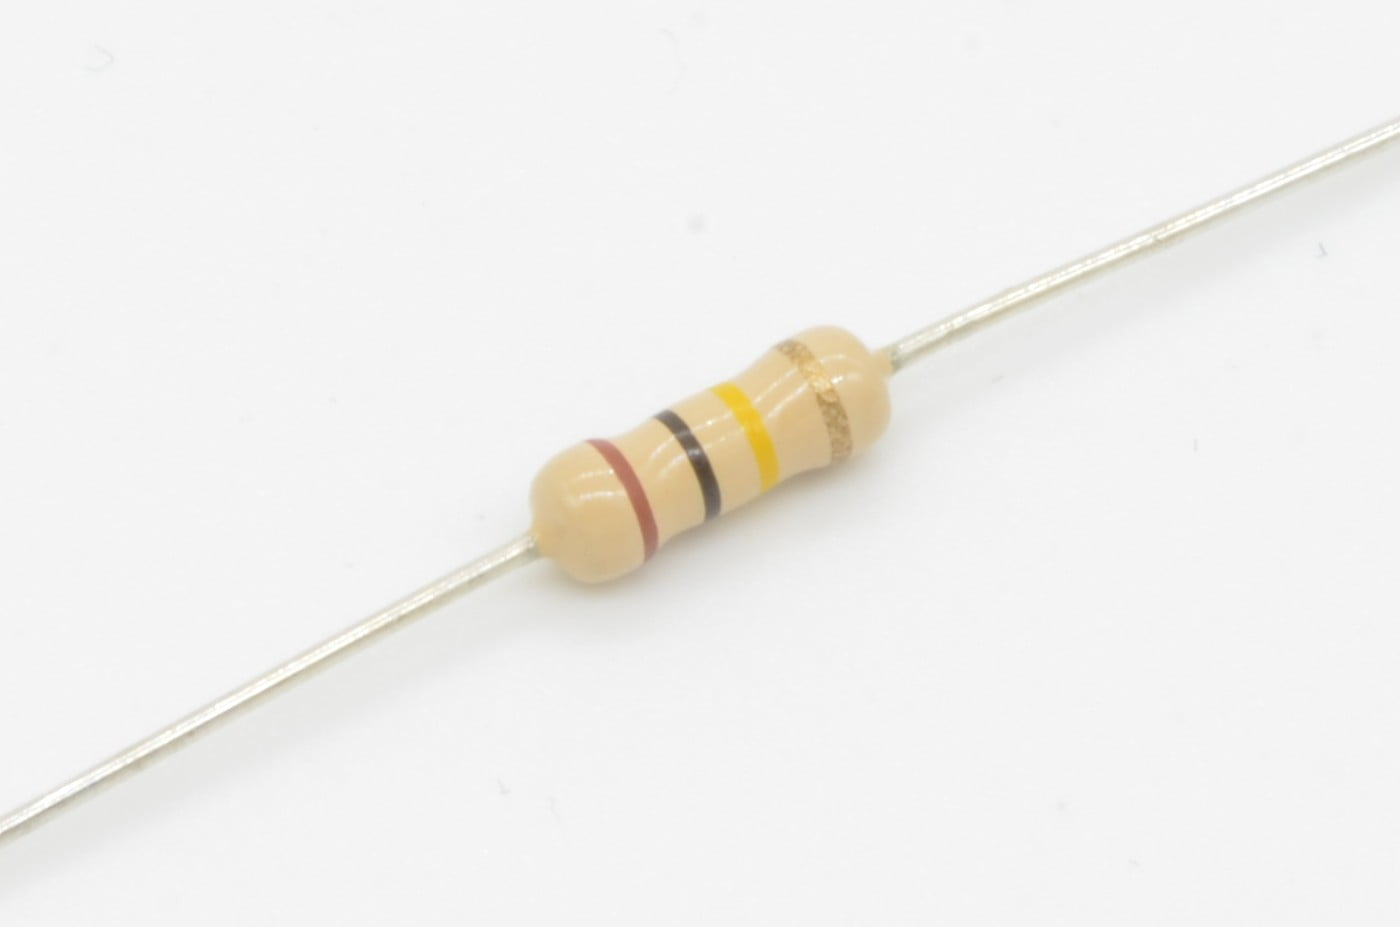
\includegraphics[width=0.6\linewidth]{materials/100k-resistor.jpg}
        \caption{Resistencia de $100\,\mathrm{k}\Omega$.}
        \label{fig_materials:100k-resistor}
    \end{figure}

    \begin{figure}
        \centering
        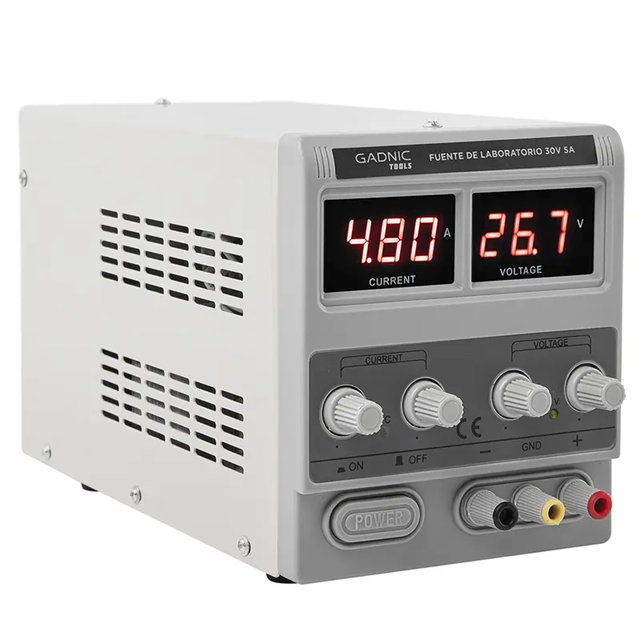
\includegraphics[width=0.6\linewidth]{materials/fuente_de_poder.png}
        \caption{Fuente de poder.}
        \label{fig_materials:fuente_de_poder}
    \end{figure}

    \begin{figure}
        \centering
        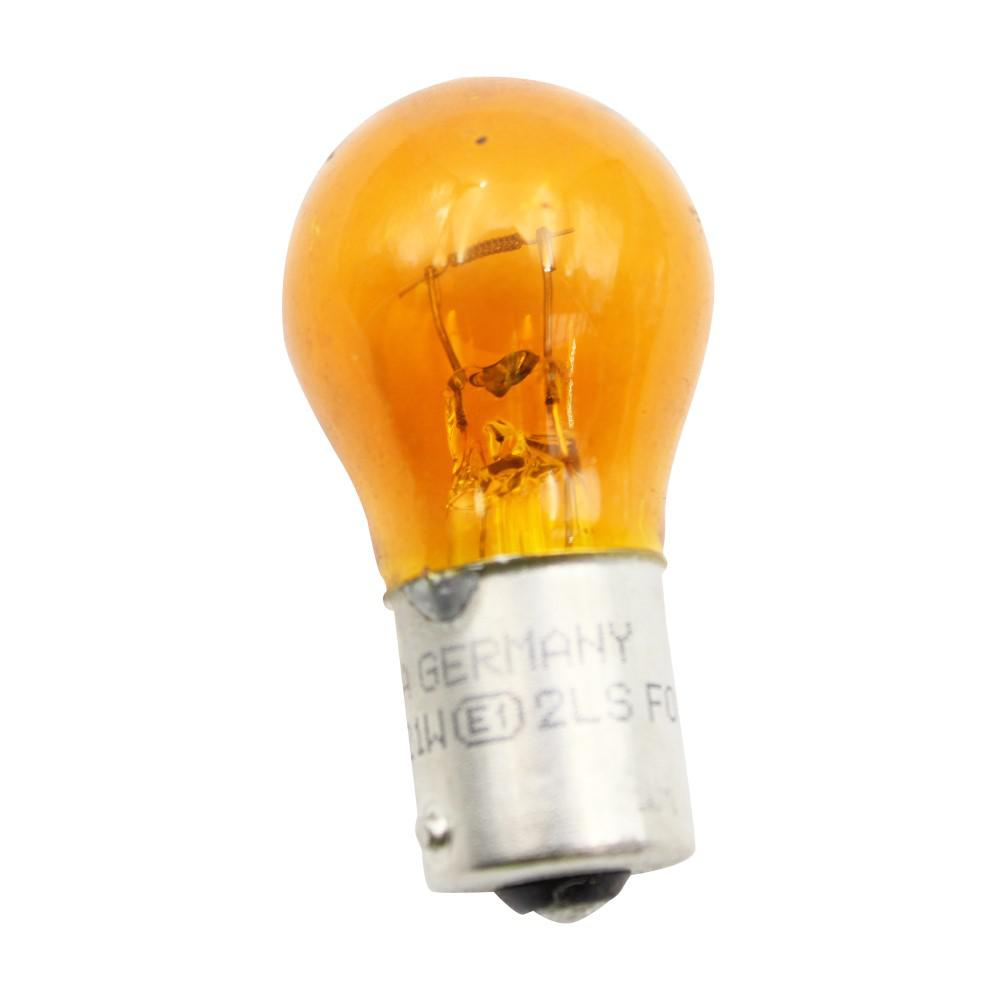
\includegraphics[width=0.4\linewidth]{materials/ampolleta.jpg}
        \caption{Ampolleta.}
        \label{fig_materials:ampolleta}
    \end{figure}
  
    \begin{figure}
        \centering
        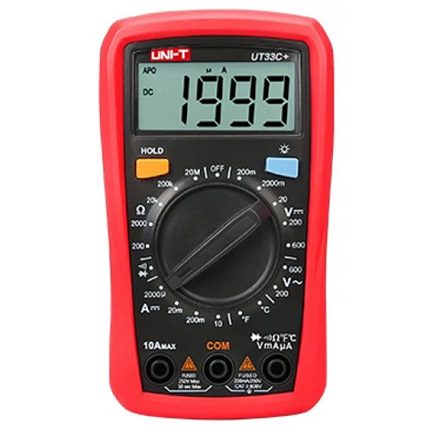
\includegraphics[width=0.6\linewidth]{materials/multitester.png}
        \caption{Multitester.}
        \label{fig_materials:multitester}
    \end{figure}

    \begin{figure}
        \centering
        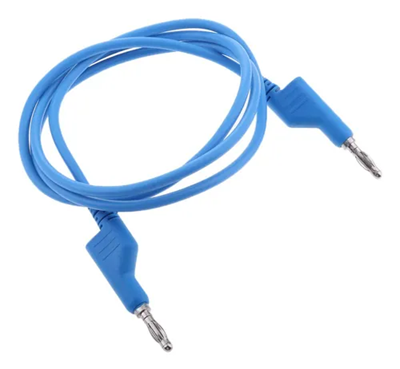
\includegraphics[width=0.6\linewidth]{materials/cables.png}
        \caption{Cables con conectores banana.}
        \label{fig_materials:cables}
    \end{figure}

    \begin{figure}
        \centering
        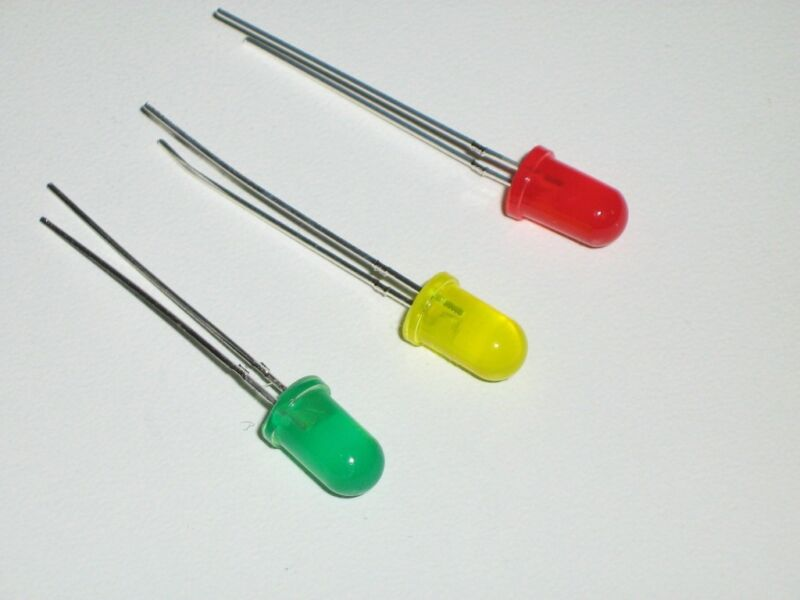
\includegraphics[width=0.6\linewidth]{materials/leds.jpg}
        \caption{LEDs de luz verde, roja y amarilla.}
        \label{fig_materials:leds}
    \end{figure}

\section{Primera experiencia.}

Buscamos distinguir entre regímenes \textbf{óhmicos} y \textbf{no óhmicos} mediante la característica $V\!-\!I$. Se registran pares $(I,V)$ para cinco dispositivos: una resistencia de $100\,\mathrm{k}\Omega$, una ampolleta y LEDs (verde, rojo y amarillo). En nuestro rango de operación, tanto la resistencia como la ampolleta exhibieron una relación $V\!-\!I$ aproximadamente \textbf{lineal} (comportamiento \textbf{óhmico}), mientras que los LEDs mostraron respuestas \textbf{no lineales} asociadas a conducción de unión \textit{p–n} con voltaje umbral.

\subsection{Procedimiento.}

\begin{enumerate}
\item Con la fuente ajustada a $0\,\mathrm{V}$, se armó el circuito de la figura~\ref{fig:p1} a fin de evitar circulación involuntaria de corriente durante el montaje y prevenir la sobrecarga. Para referencia, se adopta el sentido de circulación $c \rightarrow a \rightarrow b \rightarrow d \rightarrow c$ según el esquema.

\item Entre los bornes $a$ y $b$ se conectó el elemento bajo prueba $R$. En cada iteración se utilizó, en este orden: una resistencia de $100\,\mathrm{k}\Omega$, una ampolleta y LEDs de color verde, rojo y amarillo.

\item Se conectó en paralelo con $R$ un multímetro configurado como voltímetro, cuya polaridad se indica en la figura~\ref{fig:p1}.

\item Se conectó en serie con $R$ (entre los bornes $b$ y $c$) un multímetro configurado como amperímetro, con polaridad indicada en la figura~\ref{fig:p1}.

\item Se cerró el circuito. Para cada elemento $R$, se incrementó gradualmente la tensión de la fuente y se registraron $N=10$ pares de mediciones $(I,V)$ (corriente y voltaje), leyendo $V$ en el voltímetro e $I$ en el amperímetro. Finalizada cada serie, se redujo la tensión nuevamente a $0\,\mathrm{V}$, se abrió el circuito, se sustituyó el elemento y se repitió el procedimiento hasta completar las cinco series de datos.
\end{enumerate}

\begin{figure}
    \centering
    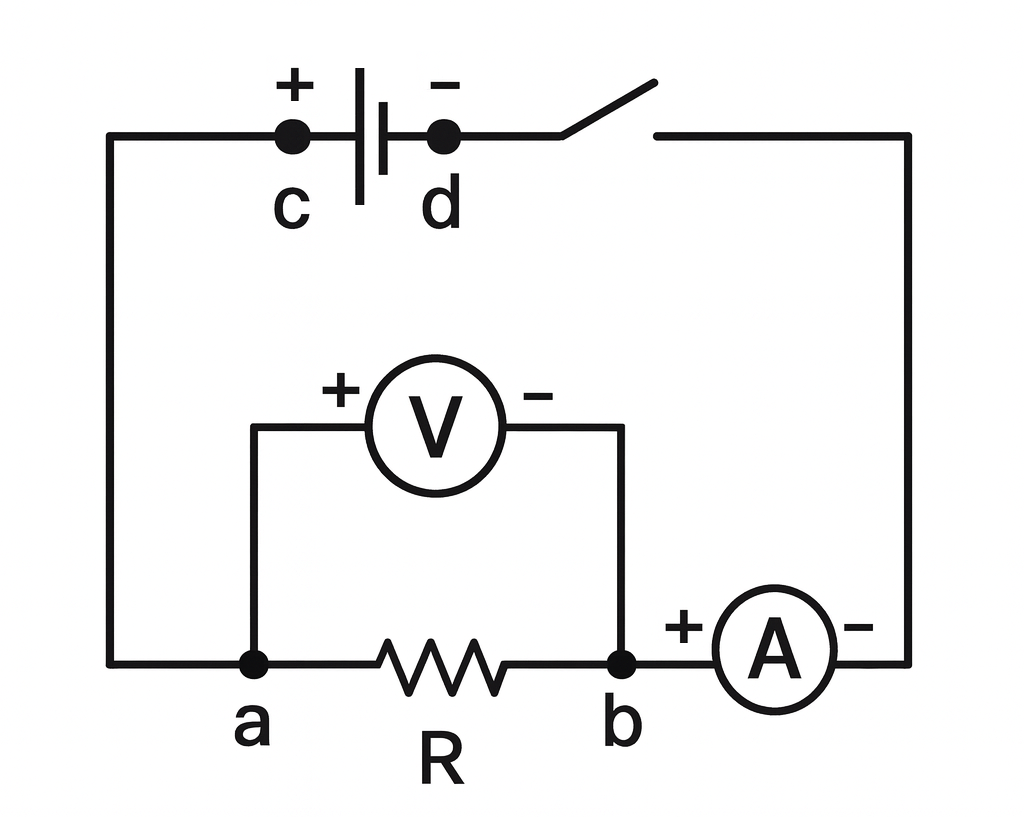
\includegraphics[width=0.8
    \linewidth]{circuit_diagram/circuito_parte1.png}
    \caption{Circuito con resistencia común.}
    \label{fig:p1}
\end{figure}

\subsection{Reporte de datos.}

Se presentan las series experimentales (10 pares $(I,V)$ por dispositivo), organizadas en \textbf{Cuadros} y ordenadas por tensión $V$ ascendente. Todas las mediciones corresponden al circuito de la Figura~\ref{fig:p1}.

\begin{itemize}
    \item Resistencia de $100\,\mathrm{k}\Omega$ (véase el Cuadro~\ref{tab1:resistencia}).
    \item Ampolleta (véase el Cuadro~\ref{tab1:ampolleta}).
    \item LED amarillo (véase el Cuadro~\ref{tab1:led_amarillo}).
    \item LED rojo (véase el Cuadro~\ref{tab1:led_rojo}).
    \item LED verde (véase el Cuadro~\ref{tab1:led_verde}).
\end{itemize}


%------------------------
% Resistencia (100 kΩ)
%------------------------

\begin{table}
\centering
\caption{Mediciones $V\!-\!I$ para la resistencia de $100\,\mathrm{k}\Omega$; 10 pares $(I,V)$ ordenados por $V$ ascendente (régimen óhmico).}

\label{tab1:resistencia}
\begin{tabular}{|c|c|c|}
\hline
$i$ & $I$ (A) & $V$ (V) \\
\hline
1  & $14.7\times 10^{-6}$ & $1.40$ \\
2  & $16.1\times 10^{-6}$ & $1.60$ \\
3  & $18.7\times 10^{-6}$ & $1.80$ \\
4  & $20.0\times 10^{-6}$ & $2.00$ \\
5  & $22.0\times 10^{-6}$ & $2.20$ \\
6  & $24.4\times 10^{-6}$ & $2.40$ \\
7  & $26.5\times 10^{-6}$ & $2.60$ \\
8  & $28.5\times 10^{-6}$ & $2.80$ \\
9  & $29.0\times 10^{-6}$ & $2.90$ \\
10 & $31.0\times 10^{-6}$ & $3.00$ \\
\hline
\end{tabular}
\end{table}

%------------------------
% Ampolleta
%------------------------

\begin{table}
\centering
\caption{Mediciones $V\!-\!I$ para la ampolleta; 10 pares $(I,V)$ ordenados por $V$ ascendente. En el rango ensayado se observa relación aproximadamente lineal (comportamiento óhmico).}
\label{tab1:ampolleta}
\begin{tabular}{|c|c|c|}
\hline
$i$ & $I$ (A) & $V$ (V) \\
\hline
1  & $0.15$ & $0.60$ \\
2  & $0.19$ & $0.95$ \\
3  & $0.24$ & $1.50$ \\
4  & $0.26$ & $1.75$ \\
5  & $0.31$ & $2.50$ \\
6  & $0.38$ & $3.40$ \\
7  & $0.39$ & $3.60$ \\
8  & $0.41$ & $4.00$ \\
9  & $0.43$ & $4.30$ \\
10 & $0.44$ & $4.50$ \\
\hline
\end{tabular}
\end{table}

%------------------------
% LED amarillo
%------------------------

\begin{table}
\centering
\caption{Mediciones $V\!-\!I$ para el LED amarillo; 10 pares $(I,V)$ ordenados por $V$ ascendente. Respuesta no lineal con umbral de conducción propio de la unión \textit{p–n}.}
\label{tab1:led_amarillo}
\begin{tabular}{|c|c|c|}
\hline
$i$ & $I$ (A) & $V$ (V) \\
\hline
1  & $0.1\times 10^{-3}$ & $1.80$ \\
2  & $0.3\times 10^{-3}$ & $1.85$ \\
3  & $0.5\times 10^{-3}$ & $1.87$ \\
4  & $0.7\times 10^{-3}$ & $1.88$ \\
5  & $1.0\times 10^{-3}$ & $1.90$ \\
6  & $1.6\times 10^{-3}$ & $1.91$ \\
7  & $2.1\times 10^{-3}$ & $1.93$ \\
8  & $2.6\times 10^{-3}$ & $1.94$ \\
9  & $3.4\times 10^{-3}$ & $1.96$ \\
10 & $6.6\times 10^{-3}$ & $1.98$ \\
\hline
\end{tabular}
\end{table}

%------------------------
% LED rojo
%------------------------

\begin{table}
\centering
\caption{Mediciones $V\!-\!I$ para el LED rojo; 10 pares $(I,V)$ ordenados por $V$ ascendente. Respuesta no lineal con umbral de conducción de la unión \textit{p–n}.}
\label{tab1:led_rojo}
\begin{tabular}{|c|c|c|}
\hline
$i$ & $I$ (A) & $V$ (V) \\
\hline
1  & $0.190\times 10^{-3}$ & $1.780$ \\
2  & $0.350\times 10^{-3}$ & $1.816$ \\
3  & $0.510\times 10^{-3}$ & $1.835$ \\
4  & $1.014\times 10^{-3}$ & $1.871$ \\
5  & $1.895\times 10^{-3}$ & $1.911$ \\
6  & $2.452\times 10^{-3}$ & $1.930$ \\
7  & $2.894\times 10^{-3}$ & $1.944$ \\
8  & $3.139\times 10^{-3}$ & $1.951$ \\
9  & $3.630\times 10^{-3}$ & $1.965$ \\
10 & $3.997\times 10^{-3}$ & $1.975$ \\
\hline
\end{tabular}
\end{table}

%------------------------
% LED verde
%------------------------
\begin{table}
\centering
\caption{Mediciones $V\!-\!I$ para el LED verde; 10 pares $(I,V)$ ordenados por $V$ ascendente. Respuesta no lineal con umbral de conducción de la unión \textit{p–n}.}
\label{tab1:led_verde}
\begin{tabular}{|c|c|c|}
\hline
$i$ & $I$ (A) & $V$ (V) \\
\hline
1  & $0.206\times 10^{-3}$ & $1.884$ \\
2  & $0.409\times 10^{-3}$ & $1.919$ \\
3  & $0.737\times 10^{-3}$ & $1.945$ \\
4  & $1.120\times 10^{-3}$ & $1.964$ \\
5  & $1.575\times 10^{-3}$ & $1.982$ \\
6  & $1.854\times 10^{-3}$ & $1.991$ \\
7  & $2.249\times 10^{-3}$ & $2.001$ \\
8  & $2.649\times 10^{-3}$ & $2.011$ \\
9  & $3.103\times 10^{-3}$ & $2.021$ \\
10 & $3.610\times 10^{-3}$ & $2.037$ \\
\hline
\end{tabular}
\end{table}

\section{Análisis de datos de la primera experiencia.}

Para cada conjunto de datos se aplicó un ajuste por mínimos cuadrados mediante \texttt{numpy.polyfit} (grado 1). El script utilizado se indica en la subsección~\ref{lst:analisis1}. Todas las unidades se expresan en SI.

%------------------------
% Modelo lineal (resistencia y ampolleta)
%------------------------
\subsection{Modelo lineal (resistencia y ampolleta)}

Para la resistencia y la ampolleta se asumió el modelo
\begin{equation*}
    V(I) = a\,I + b,
\end{equation*}
donde la pendiente $a$ (en $\Omega$) aproxima la resistencia efectiva en el rango de medición y $b$ es el offset de tensión (idealmente cercano a cero en un elemento puramente óhmico). El ajuste se realizó sobre los pares $(I,V)$ tal como fueron medidos.

Se presentan las curvas $V\!-\!I$ experimentales y sus ajustes lineales: resistencia de $100\,\mathrm{k}\Omega$ (Figura~\ref{fig:resistencia}) y ampolleta (Figura~\ref{fig:ampolleta}).

\begin{figure}
    \centering
    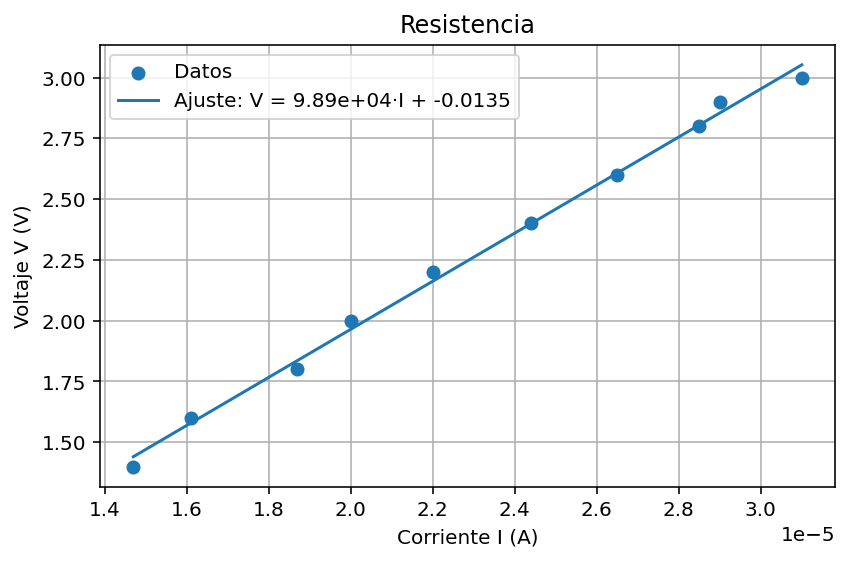
\includegraphics[width=\linewidth]{graphics_V_vs_I/Resistencia.png}
    \caption{Curva experimental $V\!-\!I$ de la resistencia y ajuste lineal $V=aI+b$.
    La pendiente entrega $R\simeq a \approx 98.9~\mathrm{k}\Omega$; el intercepto es $b$ cercano a cero.}
    \label{fig:resistencia}
\end{figure}

\begin{figure}
    \centering
    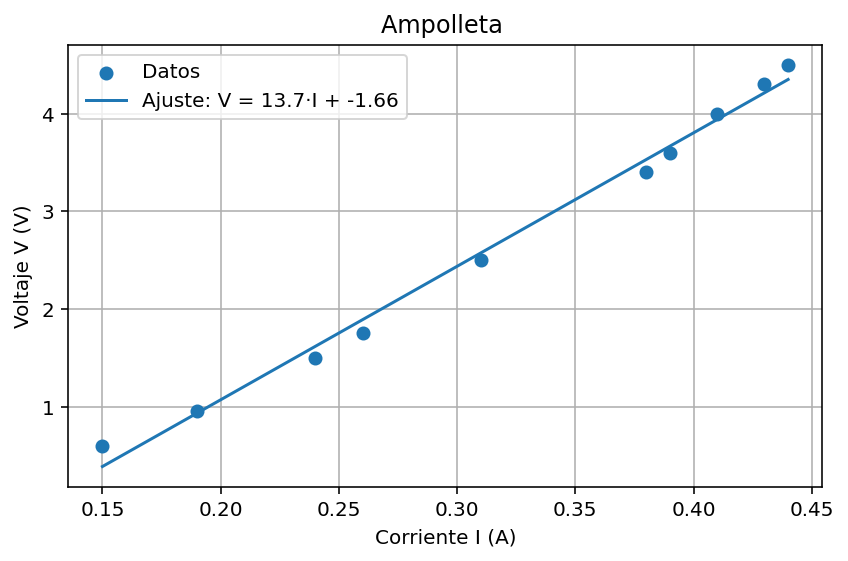
\includegraphics[width=\linewidth]{graphics_V_vs_I/Ampolleta.png}
    \caption{Curva experimental $V\!-\!I$ de la ampolleta con ajuste lineal $V=aI+b$.
    En el rango ensayado, la ampolleta se comporta aproximadamente de forma óhmica:
    $R\simeq a \approx 13.7~\Omega$ y $b \approx -1.66~\mathrm{V}$.}
    \label{fig:ampolleta}
\end{figure}

%------------------------
% Modelo semilogarítmico (LEDs)
%------------------------
\subsection{Modelo semilogarítmico (LEDs)}

Para los LEDs se empleó el modelo semilogarítmico
\begin{equation*}
    V(I) = a\,\ln I + b,
\end{equation*}
motivado por la ecuación de Shockley $I = I_s\,e^{V/(nV_T)}$ (en el régimen $I \gg I_s$), con $V_T = kT/q \approx 25.85~\mathrm{mV}$ a $25\,^\circ\mathrm{C}$.
La regresión se realizó con $\ln I$ como variable independiente, empleando únicamente puntos con $I>0$.
De la identificación $V = (nV_T)\ln I - (nV_T)\ln I_s$ se obtiene
\begin{align*}
    a \approx nV_T,&\qquad b \approx -nV_T \ln I_s,\\[6pt]
    n = \frac{a}{V_T},&\qquad I_s = e^{-b/a}.
\end{align*}
Las curvas dibujadas corresponden a evaluar el ajuste sobre un muestreo denso de $I\in[\min(I),\,\max(I)]$.

Se reportan las características $V\!-\!I$ y sus ajustes para los tres LEDs:
amarillo (Figura~\ref{fig:amarillo}), rojo (Figura~\ref{fig:rojo}) y verde (Figura~\ref{fig:verde}).

\begin{figure}
    \centering
    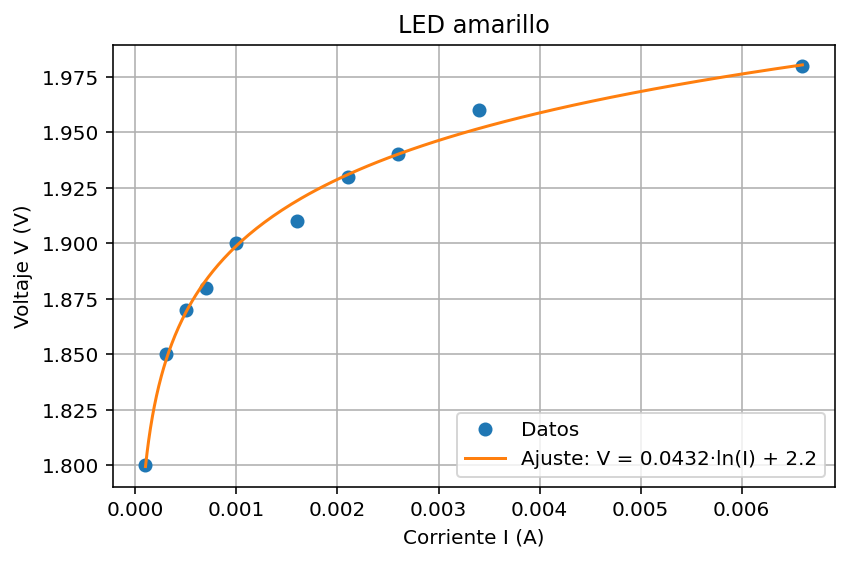
\includegraphics[width=\linewidth]{graphics_V_vs_I/LED_amarillo.png}
    \caption{Característica $V\!-\!I$ del LED amarillo graficada como $V$ vs $I$ (eje $x$ logarítmico) con ajuste $V=a\ln I+b$.
    A partir del ajuste se estiman $n\approx 1.67$ e $I_s\approx 7.9\times 10^{-23}\,\mathrm{A}$.}
    \label{fig:amarillo}
\end{figure}

\begin{figure}
    \centering
    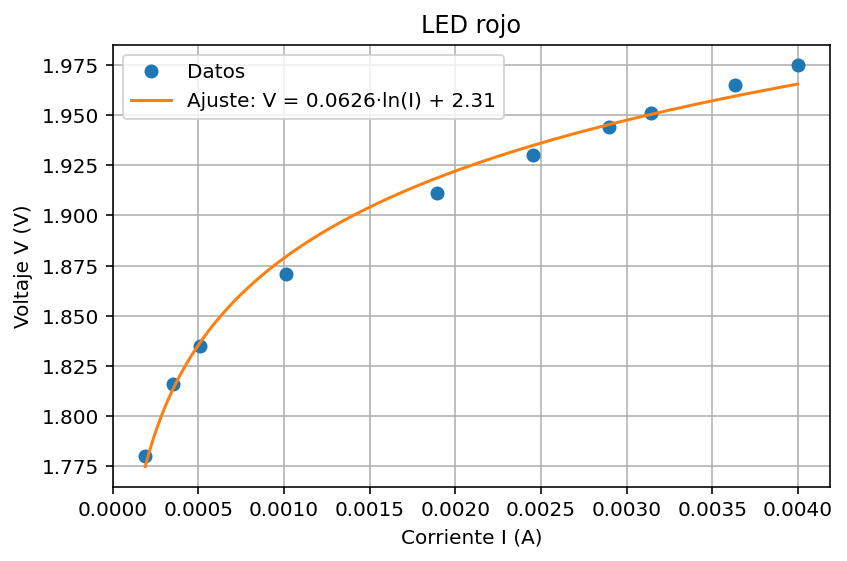
\includegraphics[width=\linewidth]{graphics_V_vs_I/LED_rojo.png}
    \caption{Característica $V\!-\!I$ del LED rojo (eje $x$ logarítmico) con ajuste $V=a\ln I+b$.
    Se obtiene $n\approx 2.42$ e $I_s\approx 9.1\times 10^{-17}\,\mathrm{A}$.}
    \label{fig:rojo}
\end{figure}

\begin{figure}
    \centering
    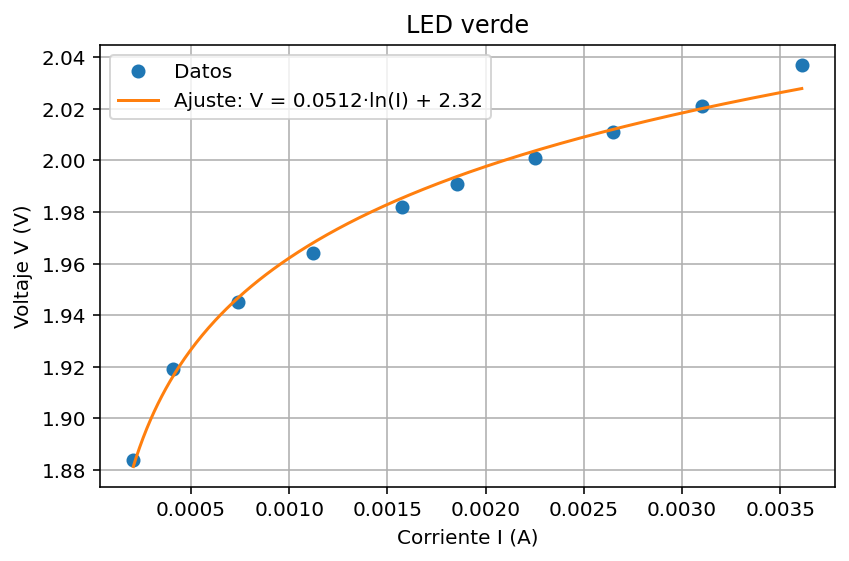
\includegraphics[width=\linewidth]{graphics_V_vs_I/LED_verde.png}
    \caption{Característica $V\!-\!I$ del LED verde (eje $x$ logarítmico) con ajuste $V=a\ln I+b$.
    Se estima $n\approx 1.98$ e $I_s\approx 2.2\times 10^{-20}\,\mathrm{A}$.}
    \label{fig:verde}
\end{figure}

\subsection{Cálculos y Script.}\label{lst:analisis1}
Los cálculos y gráficos se generaron con Python 3. 
Se usaron \texttt{numpy.polyfit} (grado 1) para los ajustes lineales, \texttt{numpy.log} para $\ln I$ y \texttt{matplotlib} para las figuras.
El script con las funciones de carga de datos, preprocesamiento (orden por $V$ y filtrado $I>0$), ajuste y graficación se puede observar{ \hypersetup{urlcolor=violet}\href{https://udeconce-my.sharepoint.com/:u:/g/personal/jrosas2022_udec_cl/EXIHjuMxI5JAr6NqEdDFxzwBYLthGC0GKXD1K0ZslACrfQ?e=y9RHvK}{aquí}}.

\subsection{Comparación de gráficos entre componentes ohmicos y no ohmicos}

La comparación de las características $V$-$I$ entre los distintos dispositivos revela diferencias fundamentales en su comportamiento eléctrico. Para la resistencia de 100 $k\Omega$, la gráfica $V$ vs $I$ muestra una relación estrictamente lineal que pasa por el origen, cumpliendo con la Ley de Ohm ideal. La ampolleta, aunque aproximadamente lineal en el rango medido, presenta una pequeña curvatura que sugiere dependencia de la resistencia con la temperatura del filamento. En contraste, los LEDs exhiben un comportamiento marcadamente no lineal característico de diodos semiconductores, con una región de conducción abrupta una vez superado el voltaje umbral (aproximadamente 1.8-2.0 $V$). Esta no linealidad se modela adecuadamente con la ecuación de Shockley, confirmando la naturaleza de unión $p$-$n$ de estos dispositivos.

\section{Segunda experiencia.}

Se estudian \textbf{redes resistivas} formadas por dos resistencias óhmicas en \textbf{serie} y en \textbf{paralelo}. El objetivo es obtener \(R_{\mathrm{eq}}=V_s/I\) a partir de pares \((I,V)\) y confrontarlo con las expresiones teóricas \(R_{\mathrm{eq,serie}}=R_1+R_2\) y \(R_{\mathrm{eq,\parallel}}=(1/R_1+1/R_2)^{-1}\), verificando la Ley de Tensiones de Kirchhoff (KVL) y la Ley de Corrientes de Kirchhoff (KCL).


\subsection{Procedimiento.}\label{sec:proc2}
\paragraph{Montaje en serie.}
\begin{enumerate}[leftmargin=*,itemsep=2pt,topsep=2pt]
  \item Con la fuente ajustada a $0\,\mathrm{V}$, se armó el circuito de la figura~\ref{fig:p2_serie} a fin de evitar circulación involuntaria de corriente durante el montaje y prevenir la sobrecarga. Se verifico la polaridad de los instrumentos: multímetro configurado como voltímetro en paralelo entre los bornes $a$ y $b$; multímetro configurado como amperímetro entre los bornes $e$ y $d$.
  
  \item Se conectaron dos resistencias $R_1$ y $R_2$ en serie, ambas de $370\,\mathrm{k}\Omega$, entre los bornes $a-b$ y $f-e$ respectivamente, que satisfacían la Ley de Ohm.
  
  \item Se calculó la resistencia equivalente teórica del conjunto:
        \begin{equation*}
            R_{\mathrm{eq,serie}}=R_1+R_2,
        \end{equation*}
        y se guardó este valor para la comparación posterior (véase el calculo en \eqref{eq:resistencia_equivalente_en_serie}).
  \item Se cerró el circuito, se aumento la de tensión de la fuente $V_i$  hasta dejarla en un valor fijo, luego se midieron:
  \begin{itemize}
      \item $V_1$ entre $a$ y $b$,
      \item $V_2$ entre $f$ y $e$,
      \item $V_0$ entre $a$ y $e$,
  \end{itemize} 
        y la corriente total $I$ en el amperímetro.
        Se registraron los datos en el Cuadro~\ref{tab:serie}.
  \item Se verificó cualitativamente la ley de Kirchhoff de tensiones: $V_i \approx V_1+V_2\approx V_0$ dentro de la incertidumbre instrumental.
\end{enumerate}

\paragraph{Montaje en paralelo.}
\begin{enumerate}[leftmargin=*,itemsep=2pt,topsep=2pt,resume]
  \item Con la fuente ajustada a 0 $V$, se desmontó el circuito anterior y se armó el circuito de la figura~\ref{fig:p2_paralelo} en paralelo con los mismos $R_1$ y $R_2$. Se mantuvo el voltímetro para medir $V_0$ en los bornes de la fuente y el amperímetro en la rama principal (entre los bornes $h$ y $b$ segun la figura~\ref{fig:p2_paralelo}).
  \item Se calculó la resistencia equivalente teórica (véase el calculo en \eqref{eq:resistencia_equivalente_en_paralelo}):
        \begin{equation*}
            R_{\mathrm{eq,\parallel}}
            =\Big(\frac{1}{R_1}+\frac{1}{R_2}\Big)^{-1}.
        \end{equation*}
  \item Se cerró el circuito y, se aumento la tensión de la fuente $V_i$ hasta dejarla en un valor fijo, luego se midieron:
    \begin{itemize}
      \item  La corriente total $I$ en el amperímetro,
      \item $I_1$ en la rama de $R_1$ (A$_1$),
      \item $I_2$ en la rama de $R_2$ (A$_2$),
    \end{itemize}
        y se registró $V_0$.
  \item Se verificó cualitativamente la ley de corrientes en el nodo: $I \approx I_1+I_2$ dentro de la incertidumbre instrumental.
\end{enumerate}

\begin{figure}
    \centering
    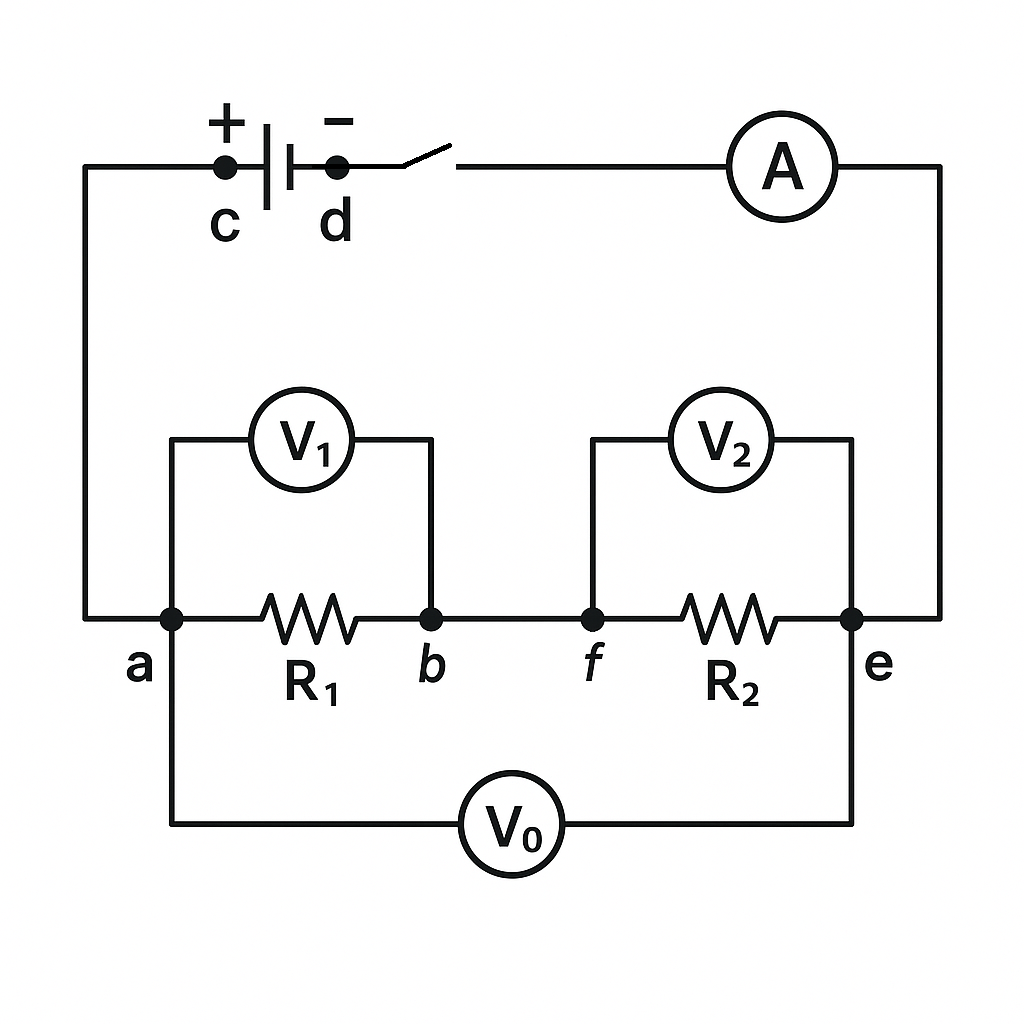
\includegraphics[width=1\linewidth]{circuit_diagram/circuito_1_parte2.png}
    \caption{Circuito de resistencias en Serie.}
    \label{fig:p2_serie}
\end{figure}

\begin{figure}
    \centering
    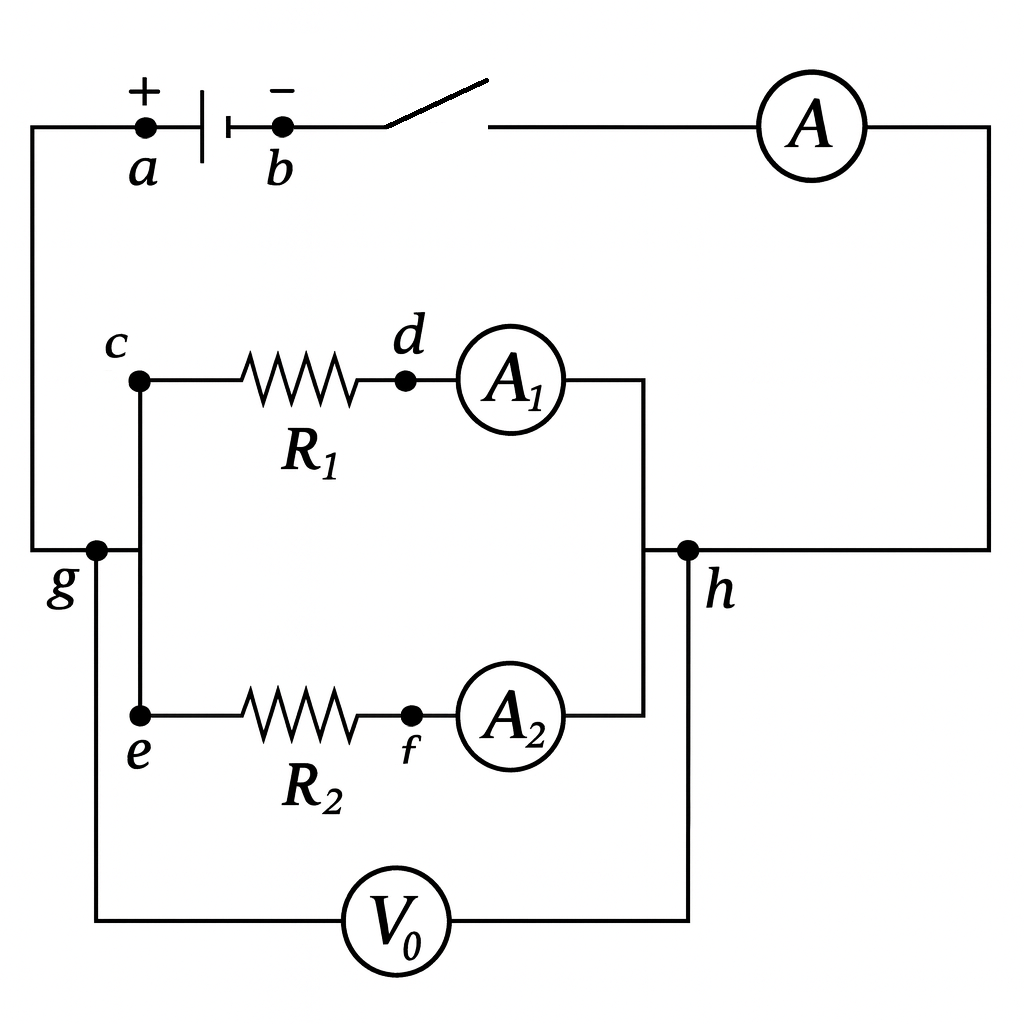
\includegraphics[width=1\linewidth]{circuit_diagram/circuito_2_parte2.png}
    \caption{Circuito de resistencias en Paralelo.}
    \label{fig:p2_paralelo}
\end{figure}

\subsection{Reporte de datos.}\label{sec:datos2}

Todas las mediciones se realizaron en corriente continua, siguiendo el conexionado indicado en las figuras de referencia. Se reportan los pares $(V_i,I)$ y las magnitudes derivadas, organizadas en \textbf{Cuadros}:

\begin{itemize}
    \item Circuito en serie (véase el Cuadro~\ref{tab:serie}).
    \item Circuito en paralelo (véase el Cuadro~\ref{tab:paralelo}).
\end{itemize}

La resistencia equivalente experimental se definió como
\begin{equation*}
    R_{\mathrm{eq,exp}} \;=\; \frac{V_s}{I_{\text{total}}},
\end{equation*}
a partir de los pares $(V_i, I_{\text{total}})$ medidos en cada montaje. Este valor se comparó con las expresiones teóricas establecidas en el procedimiento.

% --- SERIE ---
\begin{table*}
\centering
\caption{Circuito con resistencias en \textbf{serie}. Voltaje de la fuente: $V_i \approx 20.0~\text{V}$.}
\label{tab:serie}
\begin{tabular}{|c|c|c|c|c|c|c|}
\hline
$V_1$ (V) & $V_2$ (V) & $V_0$ (V) & $I_{\text{total}}$ (mA) & $R_1$ (k$\Omega$) & $R_2$ (k$\Omega$) & $R_{\text{eq}}$ (k$\Omega$) \\
\hline
9,97 & 10,02 & 20,00 & 0,0272 & 370 & 370 & 740 \\
\hline
\end{tabular}
\end{table*}

Cálculo teórico de la resistencia equivalente en serie (Fig.~\ref{fig:p2_serie}):
\begin{align}
R_{\mathrm{eq,\,serie}}
  &= R_1 + R_2 \label{eq:resistencia_equivalente_en_serie}\\[4pt]
  &= 370\,\mathrm{k}\Omega + 370\,\mathrm{k}\Omega \notag \\[4pt]
  &= 740\,\mathrm{k}\Omega. \notag
\end{align}

% --- PARALELO ---
\begin{table*}
\centering
\caption{Circuito con resistencias en \textbf{paralelo}. Voltaje de la fuente: $V_i \approx 10.0~\text{V}$.}
\label{tab:paralelo}
\begin{tabular}{|c|c|c|c|c|c|c|}
\hline
$I_1$ (mA) & $I_2$ (mA) & $V_i$ (V) & $I_{\text{total}}$ (mA) & $R_1$ (k$\Omega$) & $R_2$ (k$\Omega$) & $R_{\text{eq}}$ (k$\Omega$) \\
\hline
0,0270 & 0,0270 & 9,98 & 0,0545 & 370 & 370 & 185 \\
\hline
\end{tabular}
\end{table*}

Cálculo teórico de la $R_{\mathrm{eq}}$ en paralelo (Fig.~\ref{fig:p2_paralelo}):
\begin{align}
R_{\mathrm{eq,\,\parallel}}
&= \left(\frac{1}{R_1}+\frac{1}{R_2}\right)^{-1} \label{eq:resistencia_equivalente_en_paralelo} \\[4pt]
&= \left(\frac{1}{370\,\mathrm{k}\Omega}+\frac{1}{370\,\mathrm{k}\Omega}\right)^{-1} \notag \\[4pt]
&= \left(\frac{2}{370\,\mathrm{k}\Omega}\right)^{-1} \notag\\[4pt]
&= \frac{370\,\mathrm{k}\Omega}{2}
   = 185\,\mathrm{k}\Omega. \notag
\end{align}

\paragraph{Verificaciones cualitativas.}
En serie, la suma de caídas reportadas se compara con $V_i$ dentro de la resolución del voltímetro; en paralelo, se contrasta la ley de nodos $I\approx I_1+I_2$. Finalmente, se evalúa la coherencia entre $R_{\mathrm{eq,exp}}=V_i/I$ y $R_{\mathrm{eq,teo}}$ para cada montaje.
  
\section{Análisis de datos de la segunda experiencia.}
            
Con los datos de los cuadros \ref{tab:serie} y \ref{tab:paralelo}, es preciso notar que para el caso del circuito con las resistencias en serie, la resistencia equivalente será la suma de $R_1$ con $R_2$, a diferencia de lo que sucede con las resistencias en paralelo, donde se cumple exactamente la relación de la suma de la inversa de cada resistencia por separado. Esto se debe a la forma matemática de donde se deducen las sumas de resistencias.\\
Para las resistencias en serie:
\begin{align*}
    V &= IR_1+IR_2\\
    V &= I(R_1 + R_2)\\
    R_{eq} &= R_1 + R_2.\\
\end{align*}
Y en el caso de las resistencias en paralelo:
\begin{align*}
    I &= \frac{V}{R_1} + \frac{V}{R_2}\\
    I &= V \left(\frac{1}{R_1} + \frac{1}{R_2}\right)\\
    R_{eq} &= \frac{1}{R_1} + \frac{1}{R_2}.\\
\end{align*}
Ahora bien, 
\subsection{Aplicar la ley de Ohm a cada resistencia.}

\textbf{Circuito en serie:}
\begin{align*}
R_1 &= \frac{V_1}{I} = \frac{9,97\,\text{V}}{0,0272\,\text{mA}} \approx 366,5\,\text{k}\Omega \\
R_2 &= \frac{V_2}{I} = \frac{10,02\,\text{V}}{0,0272\,\text{mA}} \approx 368,4\,\text{k}\Omega
\end{align*}

\textbf{Circuito en paralelo:}
\begin{align*}
R_1 &= \frac{V_i}{I_1} = \frac{9,98\,\text{V}}{0,0270\,\text{mA}} \approx 369,6\,\text{k}\Omega \\
R_2 &= \frac{V_i}{I_2} = \frac{9,98\,\text{V}}{0,0270\,\text{mA}} \approx 369,6\,\text{k}\Omega
\end{align*}

\subsection{Aplicar la ley de Ohm al conjunto como si hubiese una sola resistencia. }

\textbf{Circuito en serie:}
\begin{align*}
R_{eq,\exp} = \frac{V_0}{I} = \frac{20,00\,\text{V}}{0,0272\,\text{mA}} \approx 735,3\,\text{k}\Omega 
\end{align*}

Comparación con teórico: 735,3\,$\text{k}\Omega$ \text{ vs } 740\,$\text{k}\Omega$ \quad (\text{error: } -0,6\%)

\textbf{Circuito en paralelo:}
\begin{align*}
R_{eq,\exp} = \frac{V_i}{I_{total}} = \frac{9,98\,\text{V}}{0,0545\,\text{mA}} \approx 183,1\,\text{k}\Omega 
\end{align*}
Comparación con teórico: 183,1\,$\text{k}\Omega$ \text{ vs } 185\,$\text{k}\Omega$ \quad (\text{error: } -1,0\%)

\subsection{Relación entre \texorpdfstring{$R_1$, $R_2$ y $R_{\mathrm{equivalente}}$}{R1, R2 y Requivalente}}
Se verifica que las relaciones teóricas se cumplen dentro del margen experimental:

\begin{itemize}
\item \textbf{Serie:} $R_{eq} = R_1 + R_2 \approx 366,5 + 368,4 = 734,9\,\text{k}\Omega$ (vs $735,3\,\text{k}\Omega$ experimental)
\item \textbf{Paralelo:} $\frac{1}{R_{eq}} = \frac{1}{R_1} + \frac{1}{R_2} \approx \frac{1}{369,6} + \frac{1}{369,6} = \frac{2}{369,6}$ $\rightarrow$ $R_{eq} \approx 184,8\,\text{k}\Omega$ (vs $183,1\,\text{k}\Omega$ experimental)
\end{itemize}

\subsection{Considerar el error asociado a las medidas. ¿A qué se atribuye la discrepancia entre lo obtenido y lo esperado, si existe?}

Las discrepancias observadas ($0,6$--$1,0\%$) pueden atribuirse a:
\begin{itemize}
\item Tolerancia de las resistencias (usualmente $\pm5\%$ para resistencias de carbón)
\item Error instrumental de los multímetros (especialmente en mediciones de corrientes muy bajas)
\item Resistencia interna de los cables y contactos
\item Aproximación en las lecturas analógicas de los instrumentos
\item Pequeñas variaciones en la temperatura durante las mediciones
\end{itemize}


\section{Discusión:}

Los ajustes lineales en resistencia y ampolleta entregan pendientes $R$ consistentes con el rango esperado; el \emph{offset} $b$ cercano a cero en la resistencia sugiere baja carga parasitaria, mientras que el $b$ de la ampolleta refleja efectos térmicos/contacto. En LED, el ajuste $V=a\,\ln I + b$ reproduce la curvatura no ohmica; los valores $n\sim 1.7\text{--}2.4$ se sitúan en el intervalo típico para diodos visibles, con $I_s$ muy pequeño. La verificación de KVL en serie y KCL en paralelo arroja discrepancias relativas $\lesssim 1\%$, atribuibles a tolerancias ($\pm 5\%$), resistencia interna de instrumentos y lectura discreta. Con incertidumbres instrumentales explícitas, la concordancia teórico–experimental es satisfactoria en ambos montajes.

\section{Conclusiones.}
\begin{itemize}
\item Se verificó la ley de Ohm $V = I\,R$ en el resistor; la resistencia $R$ obtenida por la pendiente (con su incertidumbre $\Delta R$) concuerda con el valor nominal.
\item La ampolleta fue aproximadamente óhmica en el rango ensayado; el leve \emph{offset}/curvatura $b$ es coherente con auto–calentamiento.
\item En los LED, la no–ohmicidad se describe con el ajuste semilog $V = a\,\ln I + b$, arrojando un factor de idealidad $n$ en el rango esperado y una corriente de saturación $I_s$ consistente con uniones $p$–$n$. 
\item  En los montajes en serie/paralelo, la resistencia equivalente experimental $R_{\mathrm{eq,exp}}$ difiere del valor teórico en menos de $\lesssim 1\%$, diferencia atribuible a tolerancias ($\pm 5\%$) y resolución de instrumentos.
\item  Con control de incertidumbres y verificación de KVL/KCL, los resultados son consistentes con la teoría.
\end{itemize}

\newpage{}
\onecolumn{}
\printbibliography

\end{document}
